%
% File acl2014.tex
%
% Contact: koller@ling.uni-potsdam.de, yusuke@nii.ac.jp
%%
%% Based on the style files for ACL-2013, which were, in turn,
%% Based on the style files for ACL-2012, which were, in turn,
%% based on the style files for ACL-2011, which were, in turn,
%% based on the style files for ACL-2010, which were, in turn,
%% based on the style files for ACL-IJCNLP-2009, which were, in turn,
%% based on the style files for EACL-2009 and IJCNLP-2008...

%% Based on the style files for EACL 2006 by
%%e.agirre@ehu.es or Sergi.Balari@uab.es
%% and that of ACL 08 by Joakim Nivre and Noah Smith

\documentclass[11pt]{article}
\usepackage{acl2014}
\usepackage{times}
\usepackage{url}
\usepackage{latexsym}
\usepackage[backend=bibtex]{biblatex}
\usepackage{graphicx}
\addbibresource{citations}


%\setlength\titlebox{5cm}

% You can expand the titlebox if you need extra space
% to show all the authors. Please do not make the titlebox
% smaller than 5cm (the original size); we will check this
% in the camera-ready version and ask you to change it back.


\title{MIM QA System}

\author{Antariksh Bothale \\
  {\tt abothale@uw.edu} \\\And
  Julian Chan\\
  {\tt jchan3@uw.edu} \\\And
  Yi-shu Wei\\
  {\tt yishuwei@uw.edu}}

\date{}

\begin{document}
\maketitle
\begin{abstract}
We detail all the work done on MIM, our Question Answering system. We describe the architecture and design choices of our system, along with a detailed description of the various NLP and information retrieval techniques used to improve MRR scores, such as query reformulation, question classification, web-boosting, answer re-ranking, and so on. We report Lenient/Strict MRR scores of 0.390/0.269 and 0.416/0.267 on the development and evaluation data sets, respectively.


\end{abstract}

\section{Introduction}
This document reports the creation and performance of an end-to-end Question Answering system called MIM that answers questions based on documents from the AQUAINT (1 or 2) corpus. We have the complete system in place for the overall task. The techniques that our system utilizes include question classification, web-boosting, answer re-ranking, and so on.

In Section 2, we present the overall architecture of MIM. In Section 3, we document the approaches and design choices in building the system. Section 4 reports final results (MRR scores) on the development and evaluation (TREC 2006 and 2007) data, together with error analysis.

\section{System Overview}

Our system architecture can be broken down into three major classes---MainFacilitator, TaskExecutor, and Session. Each question and answering session is represented by a Session object. For each session, the MainFacilitator runs the TaskExecutor(s) in sequence to produce the answers. 

The three key tasks in the pipeline, viz. Document Retrieval, Passage Retrieval and Answer Processing, are each handled by a TaskExecutor. MainFacilitator creates a new Session object runs each of the TaskExecutor(s) sequentially. Barring any execution error, the answer will be written to the Session object. 

The SystemEvaluator reads in all the question from the data set and invokes MainFacilitator. It then reads the answer from the returned Session object and writes to the output file.

The schematic diagram of our system is shown in Figure \ref{classdiagram}.

We were also able to cut down our evaluation time dramatically by running the sessions in parallel on the Condor computing cluster. 



\begin{figure}[h]
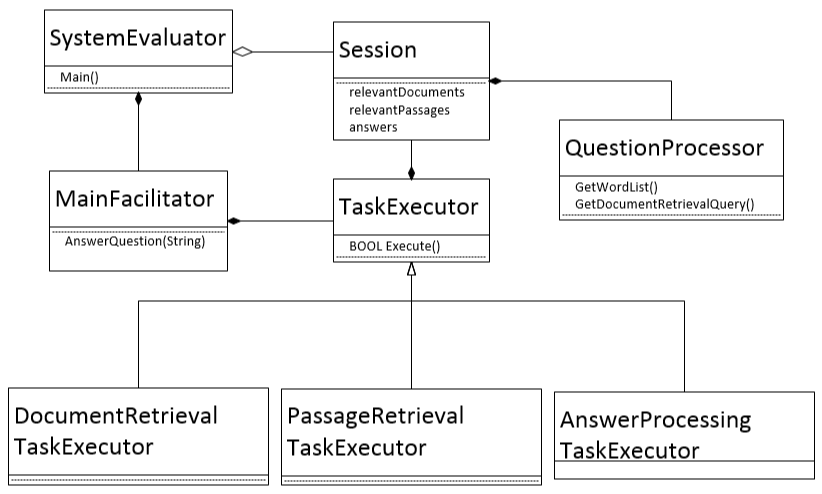
\includegraphics[width=3in,height=1.75in]{MIM_class_diagram.png}

\caption{\label{classdiagram}Class diagram of the MIM QA system}
\end{figure}


\section{Approach}
\subsection{Question Classification}
We build an SVM classifier that classifies a given question into one of the question types defined in the UIUC question taxonomy \cite{li2002learning}. The classifier uses unigrams as well as the {\it Wh-} words and the headwords as features. (Headwords are extracted from parsing the questions using the Berkeley parser \cite{berkeleyparser}).

We train the classifier on the dataset from \cite{uiuc} with 5500 labeled questions, and test the classifier on TREC 2004 and 2005 question-answering data. Since the test data are only labeled for coarse-grained question types (6 classes), we can only evaluate the classifier with coarse-grained classification, for which our SVM classifier achieves 87\% accuracy. However, for our end-to-end system we retrained the classifier for fine-grained question classification (50 classes) because coarse-grained class label does not provide sufficient information for selecting correct answers.

\subsection{Query Formation}
In this step we convert the question into a query that can be used for document retrieval. The query indicates that the subsequent module should search for the question terms in the body text, and for the target words either in the title or the body text. We also expand the query in two ways as described below in order to increase the recall of document retrieval.

\subsubsection{Morphology-Based Query Expansion}
We first expand our query with verb conjugation. To achieve this, we use a dictionary of conjugations of over 8,000 verbs from NodeBox Linguistics \cite{nodebox}. (According to the documentation, the dictionary is converted from the tree adjoint grammar developed by UPenn.) For each verb in the question in the infinitive form, we add its past tense or 3rd person singular present tense to the query​ depending on the auxiliaries in the question. If there is no auxiliary in the question, we do not add any verb conjugations.

\subsubsection{Redundancy-Based Web-Boosting}
We implemented another query expansion strategy using redundancy-based web-boosting. The original question (together with the target words) is passed to the Ask.com search engine and the snippets of the first 40 results are extracted. From these snippets we obtain bigram counts and keep only the top 10 most frequent ones that do not contain any words from the original question. Often times, we found these top bigrams to  contain the correct answer to the questions.

We then harvest unique terms from these top bigrams and add them to the query. We were able to increase our accuracy significantly (at least 10 points).

\subsection{Document Retrieval}
The Document Retrieval system takes a document retrieval query from the Query Formation step and returns a list of documents from the indexing and retrieval engine, as described below. This list of documents is then used for Passage Retrieval and Answer Processing.

\subsubsection{Indexing and Retrieval Engine}
For our indexing and retrieval engine, we use Whoosh \cite{whoosh}, which is pure-Python based text indexing, search, and spell checking library. The choice of a Python based library above alternatives such as Lucene and Indri/Lemur was motivated by its ease of integration and use with our Python code-base, and its functionality being comparable to that of its Java counterparts.

\subsubsection{Indexing Strategy}
The Beautiful Soup XML parser \cite{bsoup} was used to parse all the documents and extract the Document ID, Headline and Body Text. Whoosh's in-built indexing engine was used to index all the documents present in the corpus. The current system uses Whoosh's default indexing mechanism, which does not process the text. The indexing schema was designed to store the Document ID and Headline with the Index, while the Body Text was indexed but not stored as it would have caused unnecessary duplication of data. Instead, the text is retrieved from the document using the Document ID whenever needed.

\subsubsection{Retrieval Strategy}
For each question, the documents are ranked by the Okapi BM25F scores against the query formulated in the Query Formation step above. The 100 documents with the highest BM25F scores are returned and passed down to the subsequent step (Passage Retrieval).

\subsection{Passage Retrieval}
This step reads the documents retrieved in the last step, extracting all passages in the documents that contain the keywords (the target words, the words in the question, and the words added from web-boosting). A ``passage'' in our current system is simply defined as a sentence, where sentence segmentation is handled by Whoosh. These passages are then scored based on the density of keywords in the passage. The passage extraction and scoring function are taken from Whoosh, which are originally used for returning snippets for search results.

Since we noticed that some documents are repeated in the corpus, we filter out duplicate passages which helps to increase our recall.

Additionally, we re-ranked the retrieved passages based on a bigram-match score, which is obtained by counting the number of bigram matches the target passage has with the original question, target words and  top-10 web bigrams. Passages with higher match number are ranked higher.

\subsection{Answer Processing}
We do re-ranking based on pattern matching and the question classification result from the previous subsystem, and then chop off anything after 250 characters. If the question is classified to be of type \emph{HUM}, any answer with named entities of type \emph{PERSON} (as classified by NLTK) in the first 250 characters are bumped above answers without such entities. Likewise, if the question is classified to be of type \emph{LOC}, any answer with named entities of type \emph{GPE} or \emph{LOCATION} in the first 250 characters are bumped above answers without such entities. 

For questions of type \emph{NUM:date}, answers that have a pattern match with a date/year pattern are bumped up. 

Finally, for questions of type \emph{NUM}, we prioritize answers with numerical patterns in them. 

If there are multiple answers that satisfy any of the above criteria, we do not break ties between them and return them in the relative order in which they were returned by the passage retrieval system.

\section{Results and Discussion}
\label{sec:discussion}

With top 20 answers for each question, the above-described system attains an MRR score of 0.269 under the strict evaluation scheme (0.390 under the lenient evaluation scheme) on the development (TREC 2006) data. On the final evaluation (TREC 2007) data, the system attains a strict score of 0.267 and a lenient score of 0.416.

\subsection{Strategies that Are Most Helpful}
We noticed three strategies that yield the most substantial performance gain of our system: First is to include the target words in our query; second is to use the whole sentence rather than automatically generated snippets as our answers; and third is to exploit search results from the World Wide Web.

\subsection{Error Analysis}
The following statistics (Table \ref{stats}) were calculated to get a better understanding of system performance and of the sources of error. 

\begin{table}[h]
\begin{center}
\begin{tabular}{ |l |c |c| }
\hline
& Dev & Eval\\
\hline
Questions & 403 & 307\\
Questions with Gold Patterns & 386 & 290\\
Answers with Non-Zero Score & 263 & 197\\
Answers within Top 10 Candidates & 224 & 182\\
Answers at Top 1 Position & 117 & 91\\
\hline
\end{tabular}
\end{center}
\caption{\label{stats} System Statistics. 
}
\end{table}
It can thus be seen that roughly 30\% of answerable questions (defined as those the pattern is present and hence the answer for which can be verified) in both of the development and evaluation datasets are answered with a score of 1.0 (top answer correct).

The small difference between answers that have non-zero scores and answers that are in the top 10 candidates indicates that the answer re-ranking works fairly well if the answer is present in the top 20 answer candidates. 

However, since a sizable number of questions remain unanswered (no viable candidate in the top 20 candidates), it is also necessary to analyze the cause behind this.  Here, we present three questions for which our system scores 0, and our analysis as to why they fell through. These questions are all from the evaluation set, but the analysis is general and applies equally well for the development set.


\noindent \textbf{Question 1}: What is Krugman's Academic Specialty? 

\noindent \textbf{Answer}: Economics

\noindent \textbf{Analysis}: A look at the candidate answers returned by the system reveals that while the term ``economist'' was present in almost all of them, ``economics'' wasn't. Even among answers obtained using Web Search, while over-specific answer terms such as ``Keynesian'' were present, ``economics'' was very rare. This indicates the need for derivational morphology processing of some sort, although that comes with its own set of issues with over-generalization.

\noindent \textbf{Question 2}: When was CAFTA signed? 

\noindent \textbf{Answer}: May 2004

\noindent \textbf{Analysis}: The top answer returned by the system was relevant but wasn't complete---\emph{``Bush signed the CAFTA \ldots in May.''} On the other hand, web snippets contained too specific an answer---\emph{``\ldots the signing took place on May 28.''} For date-related answers, it might be useful to check if they contain the year too, and if not, to predict it using the document metadata.

\noindent \textbf{Question 3}: When was Rush Limbaugh born?

\noindent \textbf{Answer}: 1951

\noindent \textbf{Analysis}:
This is a surprisingly egregious failure of a system that otherwise performs reasonably well, particularly since almost all the cached web snippets contain the exact answer string. The source of error, in this case, turns out to be the fact that the system uses top bigrams from the web cache for query expansion. Since the year of birth occurs with a wide range of neighboring words, it does not rise to the top as part of any bigram, and is therefore missing from the reformulated query. An obvious solution is to score unigrams too, but that tends to promote a lot of spurious terms.

\section{Conclusion}
We have achieved fairly good results by improving key processes in the QA pipeline. We also realized (from our experience and also from that of other teams') that techniques like n-gram scoring only gave marginal improvement (if any) and we dropped them in favor of our current system. 

In the future, there are two components that we would like to improve on. The first is the document indexing and retrieval strategies, where we expect the recall of document retrieval will be further improved with more fuzzy matching techniques like spell checking and stemming/lemmatization. The second is answer scoring and re-ranking, where we would like to incorporate more deep, linguistically motivated techniques such as Minimal Recursive Semantics (MRS) or other semantic representations.



\section*{Acknowledgments}
We thank C.-J. Hsu for the code snippet for interfacing with Ask.com for the Web Boosting mode that he shared with all students on GoPost.

\printbibliography

\end{document}
